%! Author = stephaniemaerklin
%! Date = 30.08.2026

\begin{figure}
    \centering
    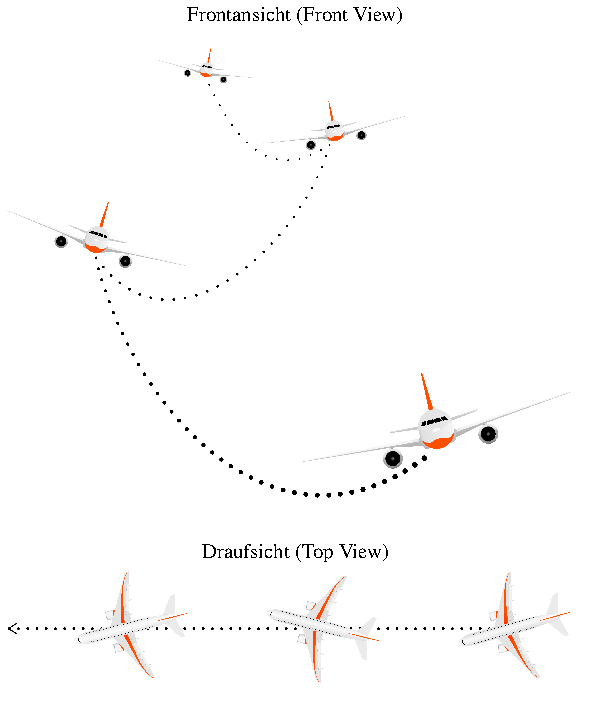
\includegraphics{papers/aircraft/images/dutchroll-transparent.pdf}
    \caption{Ablauf der Dutch Roll.
    Oben die Vorderansicht, das Flugzeug rollt abwechselnd nach rechts und
    nach links, die punktierte Linie ist die Flugbahn.
    Unten die Draufsicht, das Flugzeug fliegt von rechts nach links, die Nase
    pendelt um die Flugrichtung, das Flugzeug giert und schiebt.
    \label{aircraft:fig:dutchroll}}
\end{figure}